\documentclass{beamer}
% Language/Font package
\usepackage[utf8]{inputenc}
\usepackage[francais]{babel}
\usepackage[T1]{fontenc}

% Base package
\usepackage{graphicx}
\usepackage{color}
\usepackage{listings}
\usepackage{hyperref}

% Configuration
\definecolor{ligthYellow}{RGB}{255,255,229}

\lstset{
language=bash,
numbers=left,
numberstyle=\small,
numbersep=8pt,
basicstyle=\small\ttfamily,
tabsize=4,
showspaces=false,
showstringspaces=false,
stringstyle=\color{red}\ttfamily,
commentstyle=\color{green}\ttfamily,
breaklines=true,
frame = single,
framexleftmargin=15pt,
backgroundcolor=\color{ligthYellow}}

% Theme https://github.com/matze/mtheme
\usetheme[progressbar=frametitle]{metropolis}

% Title
\title{Présentation Git}
\subtitle{Un outil de collaboration puissant}
\date{\today}
\author{Denis Pettens \and Pablo Gonzalez Alvarez}
\institute{Louvain-li-Nux}
\titlegraphic{\hfill
\includegraphics[height=2cm]{img/logo.png}}

\begin{document}

\maketitle

\begin{frame}{Table des matières}

\setbeamertemplate{section in toc}[sections numbered]
\tableofcontents[hideallsubsections]

\end{frame}

\section{Introduction}

\begin{frame}{Gérer un projet}
Comment gérez-vous actuellement un projet ?

\begin{itemize}
    \item L'envoyer à travers un message sur Facebook, ... (\textbf{Très mauvaise idée})
    \item L'envoyer par mail (\textbf{Un peu moins})
    \item Utiliser une Dropbox, Google Drive, ... (\textbf{Déjà mieux mais toujours risqué ou manque de fonctionalités})
\end{itemize}

Solution : Utiliser un \textbf{VCS}
\end{frame}

\begin{frame}{Monsieur, c'est quoi Git?}
\begin{itemize}
    \item \texttt{Git} a été créé en 2005 par \textbf{Linus Torvalds} (auteur du kernel \texttt{Linux});
    \item Il est le logiciel de gestion de versions décentralisé (\textbf{VCS}) le plus utilisé au monde en 2016;
    \item Il permet donc de suivre dans le temps l'avancement d'un projet de son début à sa fin;
    \item Il garde en mémoire tout ce que vous avez fait un jour dans votre projet et permet de les éditer facilement;
    \item ... \footnote{Tiré en partie du site (\url{https://git-scm.com})}
\end{itemize}
\end{frame}

\begin{frame}{Pourquoi l'utiliser?}
\begin{itemize}
    \item Le plus connu et utilisé (communauté très présente);
    \item Vitesse;
    \item Conception simple;
    \item Facile d'utilisation mais aussi très puissant;
    \item Support pour les développements non linéaires (milliers de branches parallèles);
    \item Complètement distribué;
    \item Capacité à gérer efficacement des projets d'envergure tels que le noyau Linux (vitesse et compacité des données).\footnote{Tiré en partie du site (\url{https://git-scm.com})}
\end{itemize}
\end{frame}

\begin{frame}{GitKraken}
\begin{itemize}
    \item \texttt{git} ne possède pas d'interface graphique, tout se fait en ligne de commande;
    \item Simple d'utilisation;
    \item Idéale pour avoir une vue globale de son projet;
    \item Cross-plaform;
    \item Malheureusement, il n'est pas Libre.
\end{itemize}

\textbf{Autres alternatives} : \texttt{gitg}, \texttt{GitHub Desktop}, \texttt{SourceTree}, ...
\end{frame}

\begin{frame}{GtiKraken : Image}
\begin{figure}
    \centering
    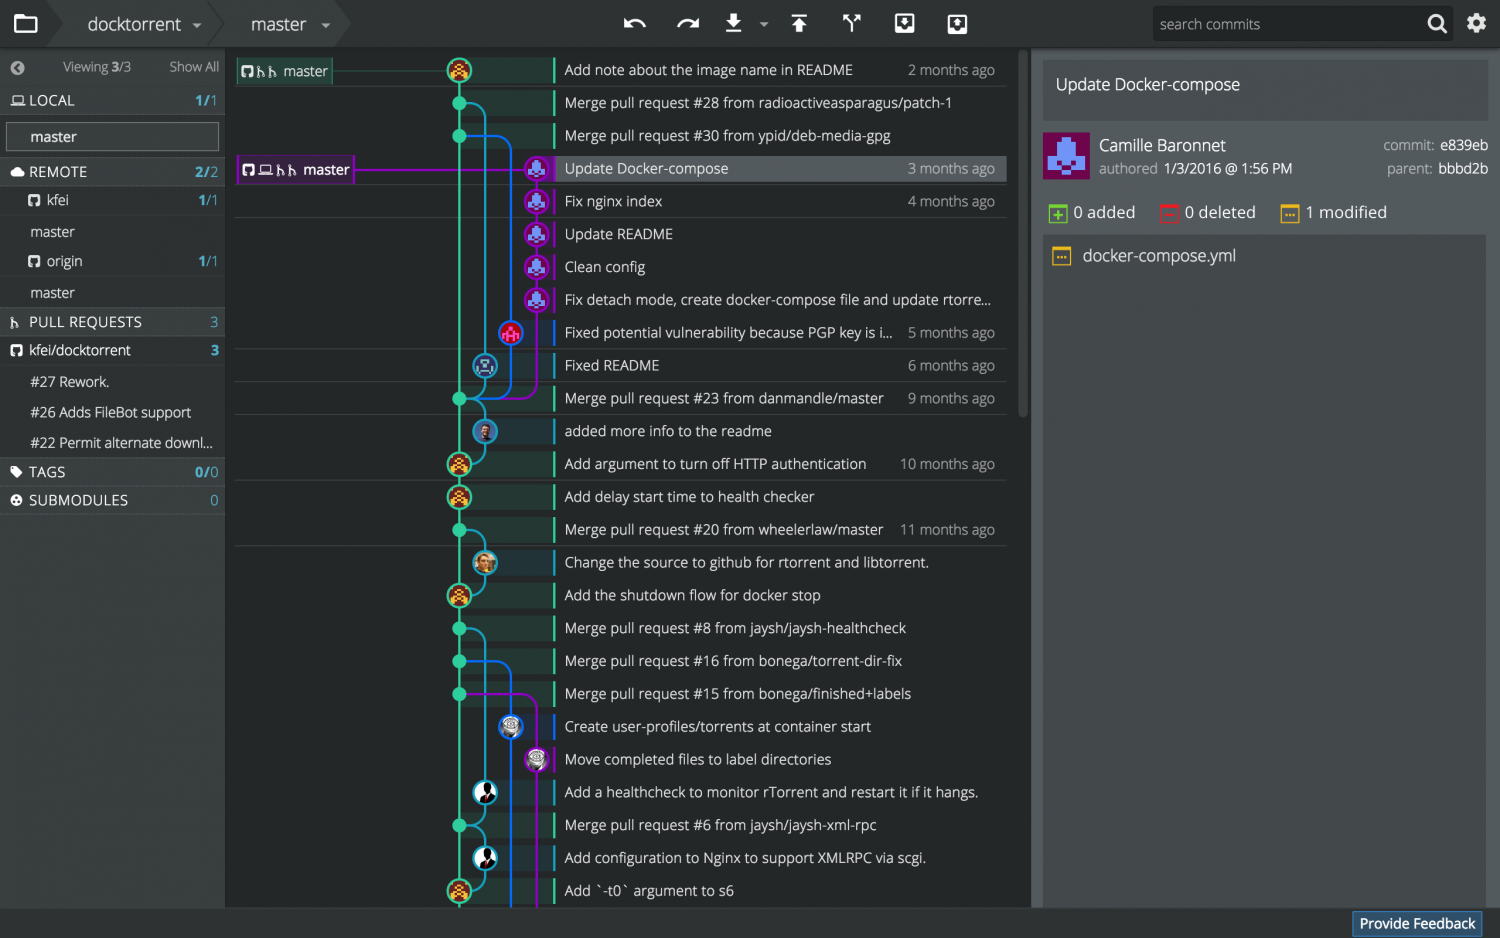
\includegraphics[height=6cm]{img/gitkraken.png}
    \caption{Tiré de \url{https://www.camillebaronnet.fr/blog/fr/gitkraken-enfin-outil-visuel-moderne-pour-git}}
\end{figure}
\end{frame}

\section{Instalation et configuration}
\begin{frame}{Installer Git et GiKraken}

\textbf{Git}
\begin{itemize}
\item \textbf{Ubuntu} : \lstinline{sudo apt-get install git}
\item \textbf{OS X} : \url{https://sourceforge.net/projects/git-osx-installer/}
\item \textbf{Windows} : \url{https://git-for-windows.github.io/}
\end{itemize}

\textbf{GitKraken}
\begin{itemize}
\item \textbf{Toutes plateformes} : \url{https://www.gitkraken.com/}
\end{itemize}
\end{frame}

\begin{frame}[fragile]
\frametitle{Configuration de base}

Git a besoin de deux informations de base sur vous pour pouvoir travailler efficacement :

\begin{itemize}
\item \textbf{Nom et Prénom}
\begin{lstlisting}
git config --global user.name "Jules Dupont"
\end{lstlisting}

\item \textbf{Email}
\begin{lstlisting}
git config --global user.email "jules.dupont@email.fr"
\end{lstlisting}
\end{itemize}

L'option \lstinline{--global} permet de configurer \texttt{git} pour tous vos autres projets sur votre PC.

GitKrakren demande de créer un compte par défaut pour pouvoir l'utiliser, ensuite il vous introduit rapidement sur son interface.
\end{frame}

\section{Premier pas avec Git}

\begin{frame}[fragile]
\frametitle{git init}

\begin{itemize}
\item Cette commande permet d'initialiser un dossier en un nouveau dépot local \texttt{git} où tout le projet versionné sera contenu dedans

\item Cela crée un sous-dossier \texttt{.git} où tout la magie de git se fait
\item Exemple
\begin{lstlisting}
mkdir newProject
cd newProject/
git init
\end{lstlisting}
\end{itemize}
\end{frame}

  \section{Les branches}
  \section{Le travail en groupe}
\begin{frame}{Les trois zones de git}
\begin{figure}
    \centering
    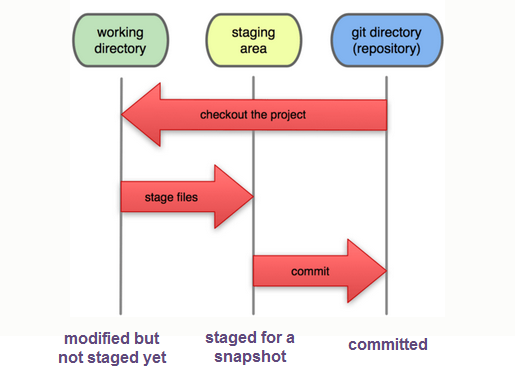
\includegraphics[height=6cm]{img/git-local-operations.png}
    \caption{Tiré du site \url{https://www.camillebaronnet.fr/blog/fr/gitkraken-enfin-outil-visuel-moderne-pour-git}}
\end{figure}
\end{frame}

\begin{frame}{Le cycle de vie d'un fichier}
\begin{figure}
    \centering
    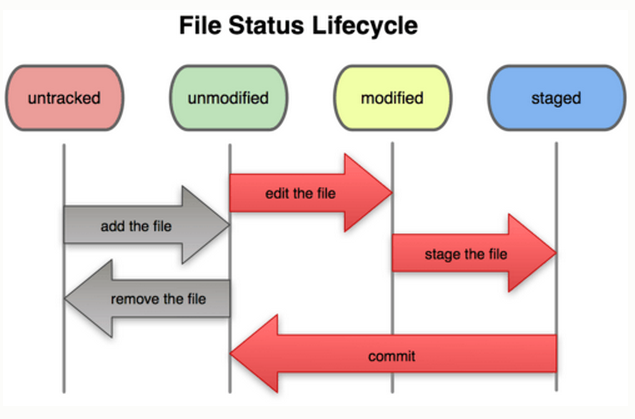
\includegraphics[height=6cm]{img/git-filestatuslifecycle.png}
    \caption{Tiré du site \url{https://www.camillebaronnet.fr/blog/fr/gitkraken-enfin-outil-visuel-moderne-pour-git}}
\end{figure}
\end{frame}

\begin{frame}[fragile]
\frametitle{git status}

\begin{itemize}
\item Cette commande permet de connaître l'état du projet sous \texttt{git}
\item Elle permet d'obtenir des informations sur les différentes zones
\item Conseil : Utiliser là dés que vous avez un doute sur l'état de votre projet
\item Exemple
\begin{lstlisting}
git status
\end{lstlisting}
\end{itemize}
\end{frame}

\begin{frame}[fragile]
\frametitle{git add}

\begin{itemize}
\item Cette commande permet d'ajouter un ou plusieurs fichier(s)/dossier(s) que l'on veut versionné(s) dans la zone de \textbf{staging} afin de préparer le prochain \textbf{commit}
\item Attention, les fichiers ne sont pas encore dans l'historique de \texttt{git}
\item Exemple
\begin{lstlisting}
touch test.txt
git add test.txt
\end{lstlisting}
\end{itemize}
\end{frame}

\begin{frame}[fragile]
\frametitle{git mv}

\begin{itemize}
\item Cette commande permet de déplacer un ou plusieurs fichier(s)/dossier(s) dans un autre dossier qui est/sont déjà versionné(s) par \texttt{git}
\item Attention, \texttt{git} suit cette modification et la place dans la zone de \textbf{staging}
\item Exemple
\begin{lstlisting}
mkdir folder
git mv test.txt folder/test.txt
\end{lstlisting}
\end{itemize}
\end{frame}

\begin{frame}[fragile]
\frametitle{git rm}

\begin{itemize}
\item Cette commande permet de supprimer un ou plusieurs fichier(s)/dossier(s) du projet qui est/sont déjà versionné(s) par \texttt{git}
\item Attention, \texttt{git} suit cette modification et la place dans la zone de \textbf{staging}
\item Exemple
\begin{lstlisting}
git rm folder/test.txt
\end{lstlisting}
\end{itemize}
\end{frame}

\begin{frame}[fragile]
\frametitle{git commit}

\begin{itemize}
\item Cette commande permet de créer un snapshot de l'état actuel du projet
\item Elle se fait généralement après des modifications de fichiers et placés dans la zone de \textbf{staging}
\item On l'identifie avec un message complet et précis
\item Exemple
\begin{lstlisting}
git commit # Ouvre l'editeur pour le message
git commit -m "Mon message"
\end{lstlisting}
\item Quand \textbf{commit} vos fichiers ?
\end{itemize}
\end{frame}

\section{Voir/Manipuler l'historique}

\begin{frame}[fragile]
\frametitle{git log}

\begin{itemize}
\item Cette commande permet de visualiser et/ou d'obtenir des informations sur les commits du projet
\item On peut remarquer que chaque commit est identifé par une clé unique qui est utile pour différentes commmandes de \texttt{git}
\item Exemple
\begin{lstlisting}
git log
\end{lstlisting}
\item Options utiles
	\begin{itemize}
		\item \lstinline{--oneline} Afficher chaque commit sur une seule ligne
		\item \lstinline{-n N} Afficher les N derniers commits 
		\item \lstinline{-p file} Afficher les commits liés à un fichier 
		\item \lstinline{-author name} Afficher les commits liés à une personne
		\item \lstinline{--pretty} et \lstinline{--graph} Affichage plus joli
	\end{itemize}
\end{itemize}
\end{frame}

\begin{frame}[fragile]
\frametitle{git diff}

\begin{itemize}
\item Cette commande permet de comparer les différences entre le \textbf{dernier commit} et votre projet actuel d'un ou de tous les fichiers
\begin{lstlisting}
git diff
git diff <file>
\end{lstlisting}

\item Pour voir celles liées à la zone de \textbf{staging}, rajoutez l'option \lstinline{--staged}
\begin{lstlisting}
git diff --staged
\end{lstlisting}

\item Pour voir entre un commit particulier et votre projet actuel ou entre deux commits
\begin{lstlisting}
git diff <commit>
git diff <commit>..<commit>
\end{lstlisting}
\end{itemize}
\end{frame}

\begin{frame}[fragile]
\frametitle{git commit --amend}

\begin{itemize}
\item Cette commande permet d'éditer le dernier commit de votre projet
\item Permet de corriger une erreur ou ajouter un fichier oublié
\item Attention, ne jamais le faire une fois le commit envoyé sur \textbf{Github} ou autre serveur
\item Exemple
\begin{lstlisting}
git commit --amend
\end{lstlisting}
\end{itemize}
\end{frame}

\begin{frame}[fragile]
\frametitle{git checkout}

\begin{itemize}
\item Cette commande permet de revenir en tant que \textbf{spectateur} sur un commit précédent
\item Attention, \texttt{git} ne modifie en rien quelque chose, vous ne faites que regarder
\item Exemple
\begin{lstlisting}
git checkout fa1751b
git checkout master # Revenir au dernier commit
\end{lstlisting}
\end{itemize}
\end{frame}

\begin{frame}[fragile]
\frametitle{git revert}

\begin{itemize}
\item Cette commande permet d'inverser un commit
\item Elle va crée un \textbf{nouveau commit} pour supprimer les changements du commit sélectionné
\item Exemple
\begin{lstlisting}
git revert fa1751b
\end{lstlisting}
\end{itemize}
\end{frame}

\begin{frame}[fragile]
\frametitle{Autres commandes utiles}

\begin{itemize}
\item \lstinline{git reset} (Commande \textbf{dangeureuse})
\item \lstinline{git rebase} (Commande \textbf{dangeureuse})
\item ...
\end{itemize}
\end{frame}

\section{Les branches}
\plain{Questions?}
\end{document}
